\documentclass{beamer}
\usepackage[latin1]{inputenc}
\usepackage{times}
\usepackage{tikz}
\usetheme{Luebeck}
%\usecolortheme{albatross}
\usepackage{amsmath,amsfonts,amsthm,amssymb}
\usepackage{setspace}
\usepackage{Tabbing}
\usepackage{fancyhdr}
\usepackage{lastpage}
\usepackage{extramarks}
\usepackage{chngpage}
\usepackage{soul,color}
\usepackage{graphicx,float,wrapfig}
\usepackage{xcolor}
\usepackage{listings}
\usepackage{float}
%\usepackage{subfloat}
\usepackage{subfig}
\usepackage{caption}
\usepackage{enumitem}
\usepackage{algpseudocode}

\definecolor{darkorange}{RGB}{240, 120, 0}

\setbeamercolor{background canvas}{bg=white}
\setbeamercolor{frametitle}{fg=white, bg=darkorange}
\setbeamercolor{normal text}{bg=black,fg=black}
\setbeamercolor{structure}{bg=black, fg=darkorange}

\title{Lecture 5: Intro To Matrix Transformations}
\date{1/28/2016}
\institute{Chris Tralie, Duke University}
\author{COMPSCI/MATH 290-04}
\begin{document}

\frame{\titlepage}

\begin{frame}{Announcements}

\begin{itemize}[label=$\blacktriangleright$]
    \item Mini Assignment 1 Part 1 Graded
    \item Part 2 Due Friday 11:55 PM
    \begin{itemize}[label=$\vartriangleright$]
        \item Only 2D required
    \end{itemize}
    \item Test Cases  %I shouldn't do too much
\end{itemize}

\end{frame}

\begin{frame}{Table of Contents}

\begin{itemize}[label=$\blacktriangleright$]
	\item Right Hand Rule Review
\end{itemize}
\begin{itemize}[label=$\vartriangleright$]
    \item Matrix Multiplication / Linear Functions
    \item 2D Matrix Transformations
    \item Rotations + Translations
    
\end{itemize}

\end{frame}

%Reviewing point above plane
\begin{frame}{Point Above Plane: Right Hand Rule}
\begin{figure}[t]
	\centering
    \includegraphics[width=0.7\textwidth]{pointAbovePlaneSketch.pdf}
\end{figure}
\end{frame}


\begin{frame}{Point Above Plane: Right Hand Rule}

\[ \vec{n} = \vec{ab} \times \vec{ac} \]

\[ \text{Test:} (\vec{ab} \times \vec{ac}) \cdot \vec{ad}\]

\begin{figure}[t]
	\centering
    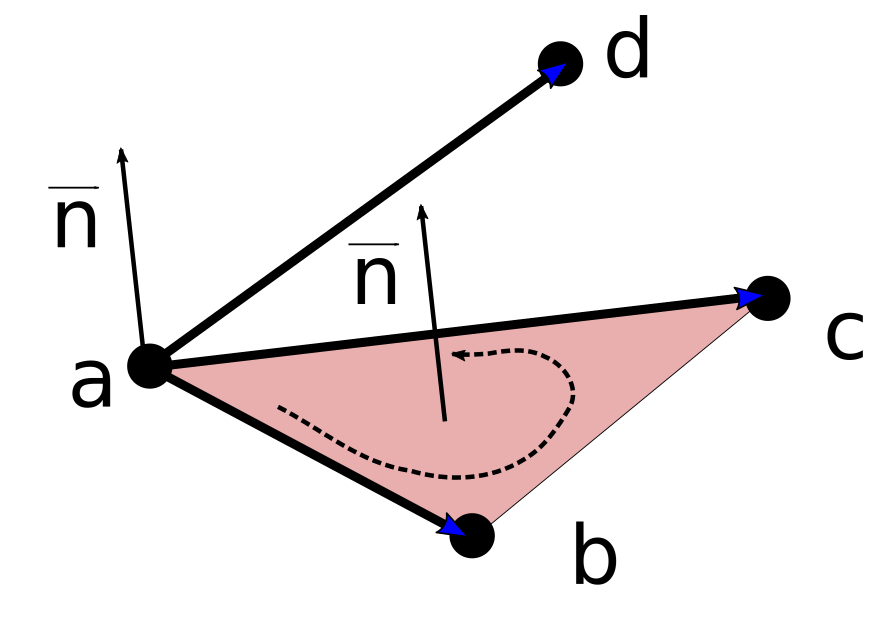
\includegraphics[width=0.7\textwidth]{pointAbovePlaneAnswer.pdf}
\end{figure}
\end{frame}

%Reviewing right hand rule with 3D stuff

\begin{frame}{Right Hand Rule Perpendicular Bisector}

\begin{figure}[t]
	\centering
    \includegraphics[width=0.7\textwidth]{3DTriangle.pdf}
\end{figure}

\end{frame}

\begin{frame}{Right Hand Rule Perpendicular Bisector}

\begin{figure}[t]
	\centering
    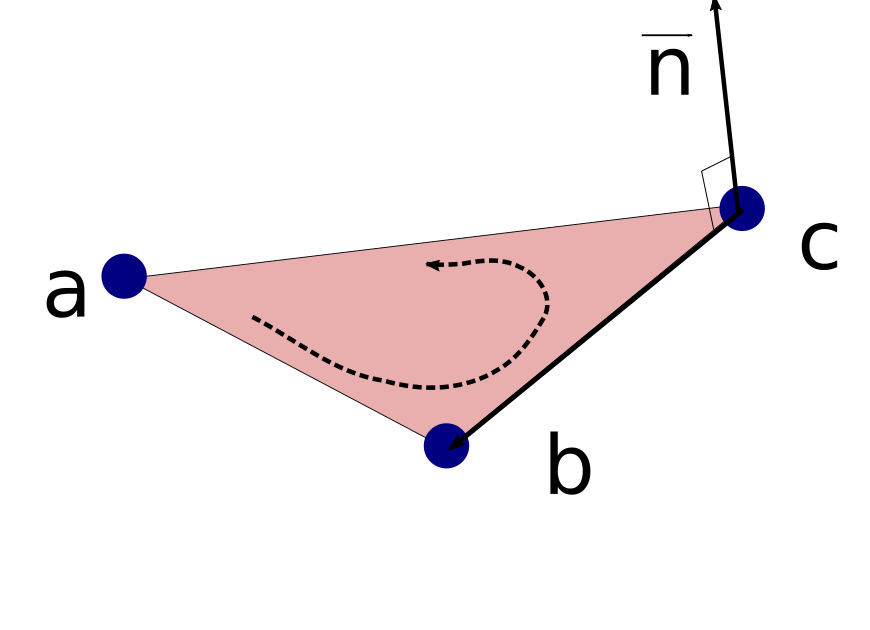
\includegraphics[width=0.7\textwidth]{3DTriangle2.pdf}
\end{figure}

\end{frame}


\begin{frame}{Right Hand Rule Perpendicular Bisector}

\begin{figure}[t]
	\centering
    \includegraphics[width=0.7\textwidth]{3DTriangle3.pdf}
\end{figure}

\end{frame}

\begin{frame}{Table of Contents}

\begin{itemize}[label=$\vartriangleright$]
	\item Right Hand Rule Review
\end{itemize}
\begin{itemize}[label=$\blacktriangleright$]
    \item Matrix Multiplication And Linear Functions
\end{itemize}
\begin{itemize}[label=$\vartriangleright$]
    \item 2D Matrix Transformations
    \item Rotations + Translations
    
\end{itemize}

\end{frame}

%%%Dot product definition with colors

\begin{frame}{Matrices And Matrix Multiplication}

\[ \left[ \begin{array}{cc} 3 & 4  \\ 3 & -3  \\ 4 & -1  \\ 0 & 2 \end{array} \right]  \left[ \begin{array}{ccc} 1 & 2 & 3  \\ -2 & 4 & 2 \end{array} \right]   =  ?  \]


\end{frame}

\begin{frame}{Matrices And Matrix Multiplication}

\[ \left[ \begin{array}{cc} 3 & 4  \\ 3 & -3  \\ 4 & -1  \\ 0 & 2 \end{array} \right]  \left[ \begin{array}{ccc} 1 & 2 & 3  \\ -2 & 4 & 2 \end{array} \right]   =  ?  \]

\[ AB_{i, j} = A_i \cdot B^j \]


\end{frame}



\begin{frame}{Matrices And Matrix Multiplication}
\[ \left[ \begin{array}{cc} \textcolor{blue}{ 3 } & \textcolor{blue}{ 4 }  \\ 3 & -3  \\ 4 & -1  \\ 0 & 2 \end{array} \right]  \left[ \begin{array}{ccc} \textcolor{blue}{ 1 } & 2 & 3  \\ \textcolor{blue}{ -2 } & 4 & 2 \end{array} \right]   =  \left[ \begin{array}{ccc} \textcolor{blue}{ -5 } & - & -  \\ - & - & -  \\ - & - & -  \\ - & - & - \end{array} \right]  \]
\end{frame}


\begin{frame}{Matrices And Matrix Multiplication}
\[ \left[ \begin{array}{cc} \textcolor{blue}{ 3 } & \textcolor{blue}{ 4 }  \\ 3 & -3  \\ 4 & -1  \\ 0 & 2 \end{array} \right]  \left[ \begin{array}{ccc} 1 & \textcolor{blue}{ 2 } & 3  \\ -2 & \textcolor{blue}{ 4 } & 2 \end{array} \right]   =  \left[ \begin{array}{ccc} -5 & \textcolor{blue}{ 22 } & -  \\ - & - & -  \\ - & - & -  \\ - & - & - \end{array} \right]  \]
\end{frame}


\begin{frame}{Matrices And Matrix Multiplication}
\[ \left[ \begin{array}{cc} \textcolor{blue}{ 3 } & \textcolor{blue}{ 4 }  \\ 3 & -3  \\ 4 & -1  \\ 0 & 2 \end{array} \right]  \left[ \begin{array}{ccc} 1 & 2 & \textcolor{blue}{ 3 }  \\ -2 & 4 & \textcolor{blue}{ 2 } \end{array} \right]   =  \left[ \begin{array}{ccc} -5 & 22 & \textcolor{blue}{ 17 }  \\ - & - & -  \\ - & - & -  \\ - & - & - \end{array} \right]  \]
\end{frame}


\begin{frame}{Matrices And Matrix Multiplication}
\[ \left[ \begin{array}{cc} 3 & 4  \\ \textcolor{blue}{ 3 } & \textcolor{blue}{ -3 }  \\ 4 & -1  \\ 0 & 2 \end{array} \right]  \left[ \begin{array}{ccc} \textcolor{blue}{ 1 } & 2 & 3  \\ \textcolor{blue}{ -2 } & 4 & 2 \end{array} \right]   =  \left[ \begin{array}{ccc} -5 & 22 & 17  \\ \textcolor{blue}{ 9 } & - & -  \\ - & - & -  \\ - & - & - \end{array} \right]  \]
\end{frame}


\begin{frame}{Matrices And Matrix Multiplication}
\[ \left[ \begin{array}{cc} 3 & 4  \\ \textcolor{blue}{ 3 } & \textcolor{blue}{ -3 }  \\ 4 & -1  \\ 0 & 2 \end{array} \right]  \left[ \begin{array}{ccc} 1 & \textcolor{blue}{ 2 } & 3  \\ -2 & \textcolor{blue}{ 4 } & 2 \end{array} \right]   =  \left[ \begin{array}{ccc} -5 & 22 & 17  \\ 9 & \textcolor{blue}{ -6 } & -  \\ - & - & -  \\ - & - & - \end{array} \right]  \]
\end{frame}


\begin{frame}{Matrices And Matrix Multiplication}
\[ \left[ \begin{array}{cc} 3 & 4  \\ \textcolor{blue}{ 3 } & \textcolor{blue}{ -3 }  \\ 4 & -1  \\ 0 & 2 \end{array} \right]  \left[ \begin{array}{ccc} 1 & 2 & \textcolor{blue}{ 3 }  \\ -2 & 4 & \textcolor{blue}{ 2 } \end{array} \right]   =  \left[ \begin{array}{ccc} -5 & 22 & 17  \\ 9 & -6 & \textcolor{blue}{ 3 }  \\ - & - & -  \\ - & - & - \end{array} \right]  \]
\end{frame}


\begin{frame}{Matrices And Matrix Multiplication}
\[ \left[ \begin{array}{cc} 3 & 4  \\ 3 & -3  \\ \textcolor{blue}{ 4 } & \textcolor{blue}{ -1 }  \\ 0 & 2 \end{array} \right]  \left[ \begin{array}{ccc} \textcolor{blue}{ 1 } & 2 & 3  \\ \textcolor{blue}{ -2 } & 4 & 2 \end{array} \right]   =  \left[ \begin{array}{ccc} -5 & 22 & 17  \\ 9 & -6 & 3  \\ \textcolor{blue}{ 6 } & - & -  \\ - & - & - \end{array} \right]  \]
\end{frame}


\begin{frame}{Matrices And Matrix Multiplication}
\[ \left[ \begin{array}{cc} 3 & 4  \\ 3 & -3  \\ \textcolor{blue}{ 4 } & \textcolor{blue}{ -1 }  \\ 0 & 2 \end{array} \right]  \left[ \begin{array}{ccc} 1 & \textcolor{blue}{ 2 } & 3  \\ -2 & \textcolor{blue}{ 4 } & 2 \end{array} \right]   =  \left[ \begin{array}{ccc} -5 & 22 & 17  \\ 9 & -6 & 3  \\ 6 & \textcolor{blue}{ 4 } & -  \\ - & - & - \end{array} \right]  \]
\end{frame}


\begin{frame}{Matrices And Matrix Multiplication}
\[ \left[ \begin{array}{cc} 3 & 4  \\ 3 & -3  \\ \textcolor{blue}{ 4 } & \textcolor{blue}{ -1 }  \\ 0 & 2 \end{array} \right]  \left[ \begin{array}{ccc} 1 & 2 & \textcolor{blue}{ 3 }  \\ -2 & 4 & \textcolor{blue}{ 2 } \end{array} \right]   =  \left[ \begin{array}{ccc} -5 & 22 & 17  \\ 9 & -6 & 3  \\ 6 & 4 & \textcolor{blue}{ 10 }  \\ - & - & - \end{array} \right]  \]
\end{frame}


\begin{frame}{Matrices And Matrix Multiplication}
\[ \left[ \begin{array}{cc} 3 & 4  \\ 3 & -3  \\ 4 & -1  \\ \textcolor{blue}{ 0 } & \textcolor{blue}{ 2 } \end{array} \right]  \left[ \begin{array}{ccc} \textcolor{blue}{ 1 } & 2 & 3  \\ \textcolor{blue}{ -2 } & 4 & 2 \end{array} \right]   =  \left[ \begin{array}{ccc} -5 & 22 & 17  \\ 9 & -6 & 3  \\ 6 & 4 & 10  \\ \textcolor{blue}{ -4 } & - & - \end{array} \right]  \]
\end{frame}


\begin{frame}{Matrices And Matrix Multiplication}
\[ \left[ \begin{array}{cc} 3 & 4  \\ 3 & -3  \\ 4 & -1  \\ \textcolor{blue}{ 0 } & \textcolor{blue}{ 2 } \end{array} \right]  \left[ \begin{array}{ccc} 1 & \textcolor{blue}{ 2 } & 3  \\ -2 & \textcolor{blue}{ 4 } & 2 \end{array} \right]   =  \left[ \begin{array}{ccc} -5 & 22 & 17  \\ 9 & -6 & 3  \\ 6 & 4 & 10  \\ -4 & \textcolor{blue}{ 8 } & - \end{array} \right]  \]
\end{frame}


\begin{frame}{Matrices And Matrix Multiplication}
\[ \left[ \begin{array}{cc} 3 & 4  \\ 3 & -3  \\ 4 & -1  \\ \textcolor{blue}{ 0 } & \textcolor{blue}{ 2 } \end{array} \right]  \left[ \begin{array}{ccc} 1 & 2 & \textcolor{blue}{ 3 }  \\ -2 & 4 & \textcolor{blue}{ 2 } \end{array} \right]   =  \left[ \begin{array}{ccc} -5 & 22 & 17  \\ 9 & -6 & 3  \\ 6 & 4 & 10  \\ -4 & 8 & \textcolor{blue}{ 4 } \end{array} \right]  \]
\end{frame}




\begin{frame}{Matrix Multiplication Observations}

\begin{itemize}[label=$\vartriangleright$]

    \item An $M \times K$ matrix time a $K \times N$ matrix is an $M \times N$ matrix
        \begin{itemize}[label=$\blacktriangleright$]
            \item Otherwise undefined
        \end{itemize}

    \item Matrix multiplication as defined takes ($M \times N \times K$) time
        \begin{itemize}[label=$\blacktriangleright$]
            \item $O(N^3)$.  Fastest known algorithm is $O(N^{2.3728639})$
        \end{itemize}

\end{itemize}

\end{frame}

\begin{frame}{Identity Matrix}

\[I_{i, j} = \left\{ \begin{array}{cc} 1 &  i = j \\ 0 & \text{otherwise} \end{array} \right\} \]

\begin{figure}[t]
	\centering
    \includegraphics[width=0.7\textwidth]{IdentityMatrix.png}
\end{figure}

\end{frame}

\begin{frame}{Identity Matrix}

Left-Handed Identity: $IA = A$

\[ \left[ \begin{array}{cccc} 1 & 0 & 0 & 0 \\ 0 & 1 & 0 & 0 \\ 0 & 0 & 1 & 0 \\ 0 & 0 & 0 & 1 \end{array} \right] \left[ \begin{array}{cc} 3 & 4  \\ 3 & -3  \\ 4 & -1  \\  0 & 2  \end{array} \right] = \left[ \begin{array}{cc} 3 & 4  \\ 3 & -3  \\ 4 & -1  \\  0 & 2  \end{array} \right]   \]



Right-Handed Identity: $AI = A$

\[ \left[ \begin{array}{cc} 3 & 4  \\ 3 & -3  \\ 4 & -1  \\  0 & 2  \end{array} \right] \left[ \begin{array}{cc} 1 & 0  \\ 0 & 1 \end{array} \right] = \left[ \begin{array}{cc} 3 & 4  \\ 3 & -3  \\ 4 & -1  \\  0 & 2  \end{array} \right] \]


\end{frame}


\begin{frame}{What Is This Really Doing?}
%It's defining a function on vectors with four numbers (Paul's idea)

\[ \left[ \begin{array}{cc} 3 & 4  \\ 3 & -3  \\ 4 & -1  \\  0 & 2  \end{array} \right]  \left[ \begin{array}{c} x  \\ y \end{array} \right]   =  \left[ \begin{array}{c} 3x + 4y  \\ 3x - 3y  \\ 4x - y  \\ 2y \end{array} \right]  \]

An $M \times N$ matrix is a {\em linear function} from $\mathbb{R}^N$ to $\mathbb{R}^M$

\end{frame}


\begin{frame}{Linear Functions}

\[ f(ax + by) = af(x) + bf(y) \]

For matrices

\[ A(aX + bY) = aAX + bAY \]

Every linear function can be written in matrix form

\end{frame}


\begin{frame}{Nonlinear Function Example}

\[ f(x, y) = x^2 + y^2 \]

\[ \mathbb{R}^2 \rightarrow \mathbb{R} \]

\uncover<2->{
\[ f(ax_1, ay_1) + f(bx_2, by_2) = a^2x_1^2 + a^2y_1^2 + b^2x_2^2 + b^2y_2^2 \]
}

\uncover<3->{
\[ f(ax_1 + bx_2, ay_1 + by_2) = a^2x_1^2 + a^2y_1^2 + b^2x_2^2 + b^2y_2^2 + \]
\[ \textcolor{red}{ 2 abx_1x_2 + 2aby_1y_2 } \]
}

\end{frame}


\begin{frame}{Nonlinear Function Example (!)}

\[ f(x) = x + 2 \]

\[ \mathbb{R} \rightarrow \mathbb{R} \]

\uncover<2->{
\begin{align} f(ax) + f(by) &= ax + 2 + bx + 2 \\ &= ax + bx + 4 \end{align}
}

\uncover<3->{
\[ f(ax + by) = ax + by + \textcolor{red}{2} \]
}

\end{frame}


\begin{frame}{Table of Contents}

\begin{itemize}[label=$\vartriangleright$]
	\item Right Hand Rule Review
    \item Matrix Multiplication And Linear Functions
\end{itemize}
\begin{itemize}[label=$\blacktriangleright$]
    \item 2D Matrix Transformations
\end{itemize}
\begin{itemize}[label=$\vartriangleright$]
    \item Rotations + Translations
    
\end{itemize}

\end{frame}



\begin{frame}{2D Scale X}

\[ \left[ \begin{array}{cc} 2 & 0 \\ 0 & 1 \end{array} \right] \left[ \begin{array}{c} x \\ y \end{array} \right] =  \left[ \begin{array}{c} 2x \\ y  \end{array} \right] \]

\begin{figure}[t]
    \captionsetup[subfloat]{labelformat=empty}
	\centering
	\subfloat[Before]{
	    \includegraphics[width=0.46\textwidth]{2DShearOrig.pdf}
	}
	\subfloat[After]{
	    \includegraphics[width=0.46\textwidth]{2DScaleX.pdf}
	}
\end{figure}

\end{frame}


\begin{frame}{2D Scale Y}

\[ \left[ \begin{array}{cc} 1 & 0 \\ 0 & 2 \end{array} \right] \left[ \begin{array}{c} x \\ y \end{array} \right] =  \left[ \begin{array}{c} x \\ 2y  \end{array} \right] \]

\begin{figure}[t]
    \captionsetup[subfloat]{labelformat=empty}
	\centering
	\subfloat[Before]{
	    \includegraphics[width=0.46\textwidth]{2DShearOrig.pdf}
	}
	\subfloat[After]{
	    \includegraphics[width=0.46\textwidth]{2DScaleY.pdf}
	}
\end{figure}

\end{frame}

\begin{frame}{2D Shear X}

\[ \left[ \begin{array}{cc} 1 & 1 \\ 0 & 1 \end{array} \right] \left[ \begin{array}{c} x \\ y \end{array} \right] =  \left[ \begin{array}{c} x + y \\ y  \end{array} \right] \]

\begin{figure}[t]
    \captionsetup[subfloat]{labelformat=empty}
	\centering
	\subfloat[Before]{
	    \includegraphics[width=0.46\textwidth]{2DShearOrig.pdf}
	}
	\subfloat[After]{
	    \includegraphics[width=0.46\textwidth]{2DShearX.pdf}
	}
\end{figure}

\end{frame}


\begin{frame}{2D Shear Y}

\[ \left[ \begin{array}{cc} 1 & 0 \\ 1 & 1 \end{array} \right] \left[ \begin{array}{c} x \\ y \end{array} \right] =  \left[ \begin{array}{c} x \\ x + y \end{array} \right] \]

\begin{figure}[t]
    \captionsetup[subfloat]{labelformat=empty}
	\centering
	\subfloat[Before]{
	    \includegraphics[width=0.46\textwidth]{2DShearOrig.pdf}
	}
	\subfloat[After]{
	    \includegraphics[width=0.46\textwidth]{2DShearY.pdf}
	}
\end{figure}

\end{frame}


\begin{frame}{2D Flip X}

\[ \left[ \begin{array}{cc} -1 & 0 \\ 0 & 1 \end{array} \right] \left[ \begin{array}{c} x \\ y \end{array} \right] =  \left[ \begin{array}{c} -x \\ y \end{array} \right] \]

\begin{figure}[t]
    \captionsetup[subfloat]{labelformat=empty}
	\centering
	\subfloat[Before]{
	    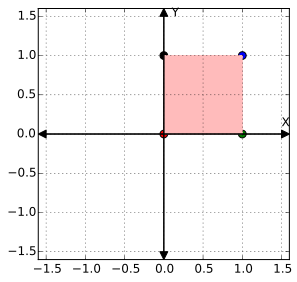
\includegraphics[width=0.46\textwidth]{2DFlipOrig.pdf}
	}
	\subfloat[After]{
	    \includegraphics[width=0.46\textwidth]{2DFlipX.pdf}
	}
\end{figure}

\end{frame}


\begin{frame}{2D Flip X And Y}

\[ \left[ \begin{array}{cc} -1 & 0 \\ 0 & -1 \end{array} \right] \left[ \begin{array}{c} x \\ y \end{array} \right] =  \left[ \begin{array}{c} -x \\ -y \end{array} \right] \]

(actually a rotation by $\pi$ about the origin)

\begin{figure}[t]
    \captionsetup[subfloat]{labelformat=empty}
	\centering
	\subfloat[Before]{
	    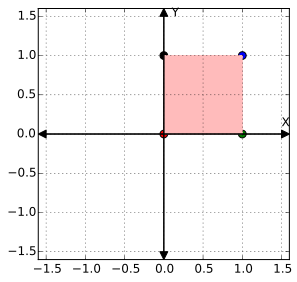
\includegraphics[width=0.46\textwidth]{2DFlipOrig.pdf}
	}
	\subfloat[After]{
	    \includegraphics[width=0.46\textwidth]{2DFlipXY.pdf}
	}
\end{figure}

\end{frame}


\begin{frame}{Matrix Compositions}

\only<1>{
\[ \left[ \begin{array}{cc} -1 & 0 \\ 0 & 1 \end{array} \right] \left[ \begin{array}{cc} 2 & 0 \\ 0 & 1 \end{array} \right] \left[ \begin{array}{c} x \\ y \end{array} \right] \]
}

\only<2-3>{
\[ \left[ \begin{array}{cc} -1 & 0 \\ 0 & 1 \end{array} \right] \left( \left[ \begin{array}{cc} 2 & 0 \\ 0 & 1 \end{array} \right] \left[ \begin{array}{c} x \\ y \end{array} \right] \right) \]
}

\only<3>{
\[ \left[ \begin{array}{cc} -1 & 0 \\ 0 & 1 \end{array} \right]   \left[ \begin{array}{c} 2x \\ y \end{array} \right] = \left[ \begin{array}{c} -2x \\ y \end{array} \right]\]
Scale, then flip

\begin{figure}[t]
    \captionsetup[subfloat]{labelformat=empty}
	\centering
	\subfloat[Before]{
	    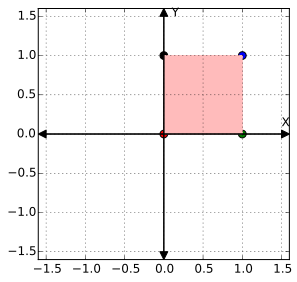
\includegraphics[width=0.46\textwidth]{2DFlipOrig.pdf}
	}
	\subfloat[After]{
	    \includegraphics[width=0.46\textwidth]{2DScaleFlip.pdf}
	}
\end{figure}
}

\end{frame}



\begin{frame}{Matrix Compositions: Associative Rule}

\only<1>{
\[ \left[ \begin{array}{cc} -1 & 0 \\ 0 & 1 \end{array} \right] \left[ \begin{array}{cc} 2 & 0 \\ 0 & 1 \end{array} \right] \left[ \begin{array}{c} x \\ y \end{array} \right] \]
}

\only<2-3>{
\[ \left( \left[ \begin{array}{cc} -1 & 0 \\ 0 & 1 \end{array} \right] \left[ \begin{array}{cc} 2 & 0 \\ 0 & 1 \end{array} \right] \right) \left[ \begin{array}{c} x \\ y \end{array} \right] \]
}

\only<3>{
\[ \left[ \begin{array}{cc} -2 & 0 \\ 0 & 1 \end{array} \right]   \left[ \begin{array}{c} x \\ y \end{array} \right] = \left[ \begin{array}{c} -2x \\ y \end{array} \right]\]
Scale, then flip

\begin{figure}[t]
    \captionsetup[subfloat]{labelformat=empty}
	\centering
	\subfloat[Before]{
	    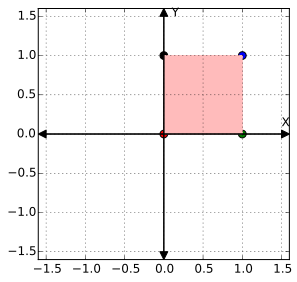
\includegraphics[width=0.46\textwidth]{2DFlipOrig.pdf}
	}
	\subfloat[After]{
	    \includegraphics[width=0.46\textwidth]{2DScaleFlip.pdf}
	}
\end{figure}
}


\end{frame}



\begin{frame}{Matrix Compositions: Commutative?}

Flip, then scale?

\only<1>{
\[ \left[ \begin{array}{cc} 2 & 0 \\ 0 & 1 \end{array} \right] \left[ \begin{array}{cc} -1 & 0 \\ 0 & 1 \end{array} \right]  \left[ \begin{array}{c} x \\ y \end{array} \right] \]
}

\only<2-3>{
\[ \left( \left[ \begin{array}{cc} -1 & 0 \\ 0 & 1 \end{array} \right] \left[ \begin{array}{cc} 2 & 0 \\ 0 & 1 \end{array} \right] \right) \left[ \begin{array}{c} x \\ y \end{array} \right] \]
}

\only<3>{
\[ \left[ \begin{array}{cc} -2 & 0 \\ 0 & 1 \end{array} \right]   \left[ \begin{array}{c} x \\ y \end{array} \right] = \left[ \begin{array}{c} -2x \\ y \end{array} \right]\]

\begin{figure}[t]
    \captionsetup[subfloat]{labelformat=empty}
	\centering
	\subfloat[Before]{
	    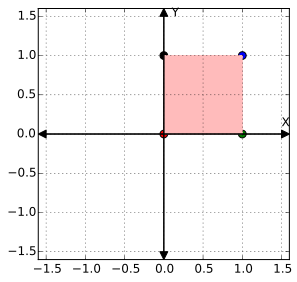
\includegraphics[width=0.46\textwidth]{2DFlipOrig.pdf}
	}
	\subfloat[After]{
	    \includegraphics[width=0.46\textwidth]{2DScaleFlip.pdf}
	}
\end{figure}
}


\end{frame}


\begin{frame}{Matrix Compositions: Commutative?}

Skew, then flip

\only<1-2>{
\[ \left( \left[ \begin{array}{cc} -1 & 0 \\ 0 & 1 \end{array} \right] \left[ \begin{array}{cc} 1 & 1 \\ 0 & 1 \end{array} \right] \right) \left[ \begin{array}{c} x \\ y \end{array} \right] \]
}

\only<2>{
\[ \left[ \begin{array}{cc} -1 & -1 \\ 0 & 1 \end{array} \right]   \left[ \begin{array}{c} x \\ y \end{array} \right] = \left[ \begin{array}{c} -x - y \\ y \end{array} \right]\]

\begin{figure}[t]
    \captionsetup[subfloat]{labelformat=empty}
	\centering
	\subfloat[Before]{
	    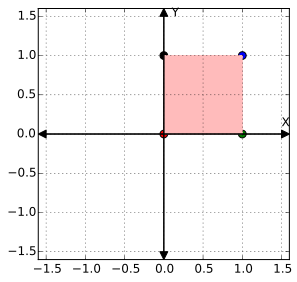
\includegraphics[width=0.46\textwidth]{2DFlipOrig.pdf}
	}
	\subfloat[After]{
	    \includegraphics[width=0.46\textwidth]{2DSkewFlip.pdf}
	}
\end{figure}
}


\end{frame}



\begin{frame}{Matrix Compositions: Commutative?}

Flip, then skew

\only<1-2>{
\[ \left( \left[ \begin{array}{cc} 1 & 1 \\ 0 & 1 \end{array} \right] \left[ \begin{array}{cc} -1 & 0 \\ 0 & 1 \end{array} \right] \right) \left[ \begin{array}{c} x \\ y \end{array} \right] \]
}

\only<2>{
\[ \left[ \begin{array}{cc} -1 & 1 \\ 0 & 1 \end{array} \right]   \left[ \begin{array}{c} x \\ y \end{array} \right] = \left[ \begin{array}{c} -x + y \\ y \end{array} \right]\]

\begin{figure}[t]
    \captionsetup[subfloat]{labelformat=empty}
	\centering
	\subfloat[Before]{
	    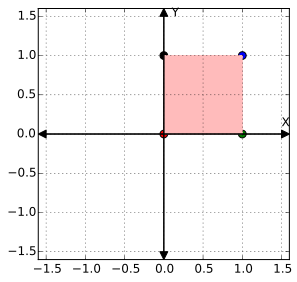
\includegraphics[width=0.46\textwidth]{2DFlipOrig.pdf}
	}
	\subfloat[After]{
	    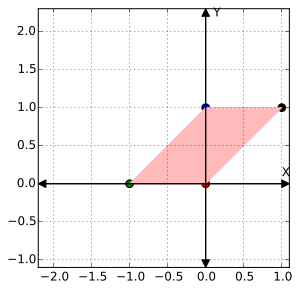
\includegraphics[width=0.46\textwidth]{2DFlipSkew.pdf}
	}
\end{figure}
}

\end{frame}

\begin{frame}{Commutativity Conclusion}

In general, matrix multiplication does not commute!

\end{frame}


\begin{frame}{Table of Contents}

\begin{itemize}[label=$\vartriangleright$]
	\item Right Hand Rule Review
    \item Matrix Multiplication And Linear Functions
    \item 2D Matrix Transformations
\end{itemize}
\begin{itemize}[label=$\blacktriangleright$]
    \item Rotations + Translations
\end{itemize}
\end{frame}


\begin{frame}{Column Vector Walking Interpretation}

\[
\left[ \begin{array}{cccccc} | & | & \vdots & | & \vdots & | \\ \vec{v_1} & \vec{v_2} & \hdots & \vec{v_k} & \hdots & \vec{v_N} \\ | & | & \vdots & | & \vdots & | \end{array}  \right] \left[ \begin{array}{c} 0 \\ 0 \\ \vdots \\ a_k \\ \vdots \\ 0 \end{array} \right] = a_k \vec{v_k}
\]

\end{frame}


\begin{frame}{Column Vector Walking Interpretation}

\[
\left[ \begin{array}{ccccccc} | & \vdots & | & \vdots & | & \vdots & | \\ \vec{v_1} & \hdots & \vec{v_k} & \hdots & \vec{v_j} & \hdots & \vec{v_N} \\| & \vdots & | & \vdots & | & \vdots & | \end{array}  \right] \left[ \begin{array}{c} 0 \\ 0 \\ \vdots \\ a_k \\ \vdots \\ a_j \\ \vdots \\ 0 \end{array} \right] = a_k \vec{v_k} + a_j \vec{v_j}
\]

\end{frame}

\begin{frame}{Column Vector Walking Interpretation}

\[
\left[ \begin{array}{cccc} | & | & \vdots & |\\ \vec{v_1} & \vec{v_2} & \hdots & \vec{v_N} \\ | & | & \vdots & | \end{array}  \right] \left[ \begin{array}{c} a_1 \\ a_2 \\ \vdots \\ a_N \end{array} \right] = \sum_{i=1}^{N} a_i \vec{v_i}
\]

Linear combination of column vectors!

\end{frame}



\begin{frame}{Column Vector Walking Interpretation}

\[ \left[ \begin{array}{cc} \textcolor{red}{-1} & \textcolor{blue}{1} \\ \textcolor{red}{0} & \textcolor{blue}{1} \end{array} \right]   \left[ \begin{array}{c} u \\ v \end{array} \right]  = \left[ \begin{array}{c} \textcolor{red}{-1} \\ \textcolor{red}{0} \end{array} \right] u + \left[ \begin{array}{c} \textcolor{blue}{1} \\ \textcolor{blue}{1} \end{array} \right] v \]

\begin{figure}[t]
	\centering
    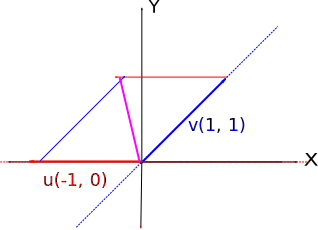
\includegraphics[width=0.7\textwidth]{ColumnVectorAdd.pdf}
\end{figure}


\end{frame}

\begin{frame}{2D Rotation Matrix Design}

\begin{figure}[t]
	\centering
    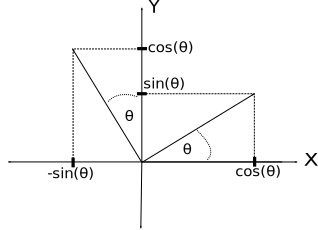
\includegraphics[width=0.6\textwidth]{ColumnVectorRot.pdf}
\end{figure}

\end{frame}

\begin{frame}{2D Rotation Matrix Design}

\begin{figure}[t]
	\centering
    \includegraphics[width=0.6\textwidth]{ColumnVectorRot2.pdf}
\end{figure}


\[ \left[ \begin{array}{cc} \textcolor{red}{\cos(\theta)} & \textcolor{blue}{-\sin(\theta)} \\ \textcolor{red}{\sin(\theta)} & \textcolor{blue}{\cos(\theta)} \end{array}  \right] \]

\end{frame}


\begin{frame}{2D Rotation Matrix: Examples}

%\[ \left[ \begin{array}{cc} \cos(\pi/2) & -\sin(\pi/4) \\ \sin(\pi/4) & \cos(\pi/4) \end{array}  \right] =   \left[ \begin{array}{cc} \cos(\pi/2) & -\sin(\pi/2) \\ \sin(\pi/4) & \cos(\pi/4) \end{array}  \right] \]

\end{frame}

%Translations: (ask them if they can come up with a matrix that does translation, and show mathematically why this is impossible using linearity.  Also show an example with the coordinate (0, 0))

\begin{frame}{Translation Matrix}

\[ f((x, y)) = (x + a, y + b) \]

\[ \mathbb{R}^2 \rightarrow \mathbb{R}^2 \]

\[  \left[  \begin{array}{cc} - & - \\ - & -  \end{array} \right] \left[ \begin{array}{c} x \\ y \end{array} \right] =  \left[ \begin{array}{c} x + a \\ y + b \end{array} \right] \]

??

\end{frame}

\begin{frame}{Homogenous Coordinates}

Pure translation with homogenous coordinates

\[ \left[ \begin{array}{ccc} 1 & 0 & T_x \\ 0 & 1 & T_y \\ 0 & 0 & 1 \end{array} \right] \left[ \begin{array}{c} x \\ y \\ 1 \end{array} \right] = \left[  \begin{array}{c}  \left[ \begin{array}{c} x \\ y \end{array} \right] + \left[ \begin{array}{c} T_x \\ T_y \end{array} \right]  \\ 1 \end{array}  \right] \]

\end{frame}

\begin{frame}{Homogenous Coordinates}

General 2D transformation + translation

\[ \left[ \begin{array}{ccc} a & b & T_x \\ c & d & T_y \\ 0 & 0 & 1 \end{array} \right] \left[ \begin{array}{c} x \\ y \\ 1 \end{array} \right] = \left[  \begin{array}{c} \left[ \begin{array}{cc} a & b \\ c & d \end{array} \right] \left[ \begin{array}{c} x \\ y \end{array} \right] + \left[ \begin{array}{c} T_x \\ T_y \end{array} \right]  \\ 1 \end{array}  \right] \]

We have some extra baggage, but we have more freedom now

\end{frame}

\begin{frame}{Group Raffle Point Question}

Write down a matrix which rotates a vector around a point

\begin{figure}[t]
	\centering
    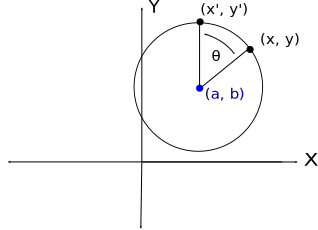
\includegraphics[width=0.5\textwidth]{RotateAroundPoint.pdf}
\end{figure}

Formulas to help you

\[ T_{(x, y)} = \left[ \begin{array}{ccc} 1 & 0 & T_x \\ 0 & 1 & T_y \\ 0 & 0 & 1 \end{array} \right], R_{\theta} = \left[ \begin{array}{ccc} \cos(\theta) & -\sin(\theta) & 0 \\ \sin(\theta) & \cos(\theta) & 0 \\ 0 & 0 & 1 \end{array} \right] \]

\end{frame}

%%%Group Raffle point question: Rotate point around a center

\begin{frame}{Javascript Sphere Plotting}

\end{frame}
%More JSON: Spherical Coordinates plotting

\end{document}

